\chapter{Metodologia}
\section{Platforma testowa}
Aby zbadać skuteczność rozpoznawania twarzy jako metody uwierzytelniającej użytkowników należało w pierwszej kolejności opracować oraz zaimplementować platformę testową. Dzięki niej w dalszej części pracy będzie możliwe przeprowadzenie badań z udziałem internautów.

% \subsubsection{Wymagania funkcjonalne i niefunkcjonalne}
% Proces określenia wymagań funkcjonalnych oraz niefunkcjoanlnych jest kluczowym aspektem w fazie projektowania systemu. Pozwala stworzyć pełen zbiór wytycznych związanych z funkcjonowaniem i działaniem systemu.

% \paragraph{Wymagania funkcjonalne}
% \begin{itemize}
%   \item Rejestracja użytkownika
%   \item Logowanie użytkownika przy pomocy tradycyjnej metody
%   \item Logowanie użytkownika przy pomocy rozpoznawania twarzy
%   \item Dostęp do podstawowych danych użytkownika
%   \item Wyświetlanie metryk 
% \end{itemize}

\subsubsection{Modele danych}
Kolejnym etapem w procesie projektowania systemu informatycznego jest opracowanie modelu danych. Pozwala to na wyselekcjonowanie niezbędnych danych do funkcjonowania systemu, które będą następnie wykorzystywane do tworzenia poszczególnych tabel lub kolecji danych. Dzięki temu możliwe jest skuteczne zaplanowanie struktury danych, na podstawie której będzie funkcjonował serwis. Ważnym aspektem jest fakt, że staranne opracowanie modelu danych pozwoli na minimalizację problemów na dalszych etapach tworzenia platformy testowej. Można wyróżnić 3 podstawowe modele danych: \emph{konceptualny}, \emph{logiczny} oraz \emph{fizyczny}. Ze względu na niski stopień skomplikowania systemu stworzony został tylko model fizyczny danych, dzięki któremu dalszy proces imlpementacji rzeczywistej aplikacji przebiegał sprawniej. 

% TODO
\begin{figure}[ht]
	\centering
		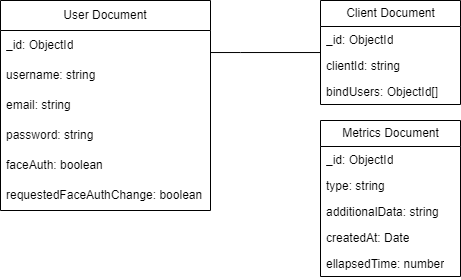
\includegraphics[width=0.5\linewidth]{imgs/db-model.png}
	\caption{Fizyczny model danych}
	\label{fig:model-danych}
\end{figure}
\subsubsection{Architektura aplikacji}
\begin{figure}[ht]
	\centering
		\includegraphics[width=1\linewidth]{imgs/Diagram bez tytułu.drawio (2).png}
	\caption{Architektura platformy testowej}
	\label{fig:architektura-aplikacji}
\end{figure}

Obecnie istnieje kilka popularnych architektur, które wykorzystywane są do budowy aplikacji internetowych. W etapie projektowania platformy zdecydowano się na wykorzystanie architektury mikroserwisowej wykorzystującej kolejkę wiadomości do komunikacji między pomniejszymi serwisami. Na początku warto zaznaczyć, że mikroserwisy cechują się bardzo dobrą skalowalnością, wykrywaniem oraz naprawianiem potencjalnych błędów w oprogramowaniu. Z uwagi na fakt wykorzystywania różnych języków programowania przy implementacji aplikacji serwerowej, wykorzystanie takiej architektury było bardzo dobrym rozwiązaniem, zapewniającym integrację serwisów na wysokim poziomie.
Analizując diagram przedstawiony na rysunku 3.1 można wyróżnić 3 główne warstwy.

\paragraph{Warstwa dostępowa} zadaniem której jest komunikacja serwisu z użytkownikiem, wykorzystując aplikację napisaną przy użyciu frameworka Angular. Przy pomocy tej warstwy użytkownik może przetestować różne metody uwierzytelniania w tym logowanie przy pomocy rozpoznawania twarzy.

\paragraph{Warstwa biznesowa} Jej zadaniem jest przetwarzanie danych otrzymanych z aplikacji dostępowej. W jej skład wchodzi kilka niezbędnych składników:
\begin{itemize}
  \item Gateway --- służy jako bramka, do oddelegowania zapytań użytkownika na określone serwisy przy pomocy kolejki wiadomości
  \item Kolejka wiadomości --- jej zadaniem jest wymiana wiadomości między dostępnymi mikroserwisami
  \item UserApp --- serwis do zarządzania użytkownikami. W jego skład wchodzą metody odpowiedzialne za tworzenie oraz pobieranie niezbędnych danych użytkowników
  \item AuthApp --- serwis zarządzający uwierzytelnianiem użytkowników zarówno tradycyjnymi metodami jak i metodami wykorzystującymi sztuczną inteligencję.
  \item ClientApp --- serwis, którego głównym zadaniem jest rejestracja urządzeń z których użytkownik się loguje do zapewnienia większego bezpieczeństwa płynącego z wykorzystania rozpoznawania twarzy.
  \item MetricsApp --- serwis który zbiera dane o czasie wykonywania procesu logowania różnymi metodami.
  \item AIApp --- serwis którego zadaniem jest przetwarzanie zdjęć użytkowników oraz udostępnianie metod do rozpoznawania twarzy.
\end{itemize}

\paragraph{Warstwa danych} Służy do przechowywania danych serwisu oraz wykonywanie operacji na bazie danych. Wykorzysuje MongoDB.
\\
Aby umożliwić uruchomienie aplikacji na dedykowanym serwerze, niezbędne było wykorzystanie narzędzia Docker. Umożliwiło to stworzenie oddzielnego środowiska wykonawczego w postaci osobnych kontenerów na każdy z utworzonych serwisów, w tym bazy danych oraz kolejki wiadomości, który mógł zostać uruchomiony na dowolnej platformie. Aby zapewnić większe bezpieczeństwo aplikacji oraz urchonić mikroserwisy przed nieuprawnionym dostępem, poszczególne aplikacje komunikują się poprzez wykorzystanie wewnętrznej sieci między kontenerami. Udostępnione zostały 2 porty, z którymi komunikować mogła się aplikacja dostępowa:
\begin{itemize}
  \item \emph{\:5000} --- port, na którym udostepniony jest serwis związany z wykorzystaniem sztucznej inteligencji do rozpoznawania twarzy
  \item \emph{\:9000} --- port, na którym udostępniona jest bramka, która oddelegowuje odpowiednie rządania poprzez kolejkę wiadomości do odpowiednich serwisów.
\end{itemize}

\subsubsection{Widoki}
Frontend platformy testowej składa się z dwóch głównych widoków oraz szeregu funkcjonalności dzięki którym mozliwe jest przetestowanie tradycyjnych metod logowania z tymi wykorzystującymi rozpoznawanie twarzy. \\
\textbf{Strona logowania} na której użytkownik może:
\begin{itemize}
   \item stworzyć nowe konto --- podając kluczowe do działania apllikacji dane oraz dodatkowo zeskanować twarz jeżeli użytkownik wyraził chęć logowania przy pomocy rozpoznawania twarzy
   \item zalogować się na konto --- wybierając jedną z dostępnych metod czyli tradycyjne logowanie hasłem oraz logowanie rozpoznawaniem twarzy z wyborem który algorytm ma zaostać wykorzystany.
\end{itemize}

\textbf{Strona panelu użtkownika} oferująca:
\begin{itemize}
  \item przeglądanie danych użytkownika --- zarówno tych podanych w procesie rejestracji jak i dodatkowe dane takie, jak zapisane przeglądarki.
  \item wylogowanie z systemu
  \item przeglądanie danych logowania --- lista danych o procesach logowania w skład których wchodzi czas oraz informacja na temat wybranej metody logowania.
\end{itemize}

% \subsubsection{Opis API}
% W serwisach internetowych obowiązującym standardem komunikacji jest protoków HTTP (ang. Hyper Text Transfer Protocol). Wykorzystuje się go do komunikacji między warstwą dostępową a warstwą biznesową, która udostępnia API (ang. Application Programming Interface). W przypadku omawianej platformy testowej można wyróżnić:
% \begin{itemize}
%   \item \emph{POST :9000/api/v1/gateway/auth/login} --- logowanie hasłowe
%   \item \emph{POST :9000/api/v1/gateway/auth/face-login} --- logowanie twarzą
%   \item \emph{POST :9000/api/v1/gateway/client/register} --- logowanie
%   \item \emph{POST :9000/api/v1/gateway/client/bind} --- logowanie
%   \item \emph{POST :9000/api/v1/gateway/client/unbind} --- logowanie
%   \item \emph{POST :9000/api/v1/gateway/auth/login} --- logowanie

% \end{itemize}

\subsubsection{Zabezpieczenia}
\paragraph{JSON Web Token} standard wymiany tokenów, zapewniający warstwę zabezpieczającą przed nieautoryzowanym dostępem do aplikacji. JWT został wykorzystany, jako kluczowy element potwierdzający, że dany użytkownik zalogował się poprawnymi danymi do systemu. Działanie mechanizmu rozpoczyna się od wykonania akcji, mającej na celu zalogowanie uzytkownika, zarówno tradycyjną metodą jak i przy pomocy rozpoznawania twarzy. W przypadku, kiedy system potwierdzi wiarygodność danego użytkownika, następuje wygenerowanie tokenu przy pomocy algorytmów kryptograficznych. Opcjonalnie można podać dane, które zostaną zapisane do takiego unikalnego tokena. Ostatnim krokiem jest wysłanie go do aplikacji dostępowej i zapisanie w pamięci przeglądarki. Sam token składa się z 3 elementów:
\begin{itemize}
  \item Header - zawiera typ tokena oraz algorytm szyfrujący
  \item Payload - zazwyczaj zawiera opcjonalne dane, zapisane programistycznie oraz długość życia tokenu
  \item Verify - podpis cyfrowy stanowiący sumę kontrolną do weryfikacji poprawności tokenu
\end{itemize}

\paragraph{Zapisywanie przeglądarki} ma na celu uniemożliwienie logowania przy pomocy rozpoznawania twarzy na urządzeniach niezaufanych. Algorytmy i sieci neuronowe, których zadaniem jest rozpoznwanie twarzy same w sobie nie są w żaden sposób zabezpieczone na różne ataki. Przykładem może być próba logowania przy pomocy zdjęcia dowolnego użytkownika, który zarejestrowany jest w systemie. Jednym z proszych w imlpementacji zabezpieczeń jest wykorzystanie zapamiętywania urządzenia (przeglądarki) użytkownika. Dzięki czemu opcja logowania przy pomocy rozpoznawania twarzy jest możliwa tylko na zaufanych urządzeniach. Sposobem na dodanie zaufanej przeglądarki jest zarejestrowanie lub zalogowanie tradycyjną metodą.


\section{Model sieci neuronowej}
\subsubsection{Dane}
Wybór odpowiedniego zbioru danych jest kluczowym elementem w procesie uczenia oraz testowania opracowanych modeli uczenia głębiokiego. Na potrzeby niniejszej pracy wykorzystany został gotowy zbiór danych \emph{CelebA Face Recognition Triplets} opracowany przez [...]. Zbiór danych składa się z pliku .csv który zawiera 16000 trójek zdjęć - Anchor, Positive, Negative oraz 45000 zdjęć twary różnych osób. Wykorzystanie gotowego zbioru danych pozwoliło zaoszczędzić czas na ręczne dobieranie i walidowanie zdjęć twarzy.
Każde zdjęcie w omawianym zbiorze ma rozmiar 224px na 224px oraz składa się z 3 kanałów kolorystycznych (R,G,B).
\subsubsection{Architektura sieci}
Opracowany model sieci jest siecią typu syjamskiego. Oznacza to, że do działania wykorzystuje 2 lub więcej identycznych podsieci uczenia głębokiego, do realizowania zadania. Takie sieci nie służą do klasyfikacji lub etykietowania zdjęć. Zazwyczaj służą do obliczania dystansu (podobieństwa) między parami zdjęć. Dlatego też tego typu sieci doskonale nadają się do realizowania zadania rozpoznawania twarzy. \\
Opracowana syjamska sieć neuronowa wykorzystuje model Xception w swoich podsieciach. Aby przyspieszyć proces implementacji, wykorzystano gotowy, wytrenowany model tej sieci z biblioteki Keras. Celem sieci Xception jest konwersja zdjęcia twarzy na postać wektorową która jest wykorzystywana na późniejszym etapie rozpoznawania twarzy.
Danymi wejściowymi dla głównej sieci są trójki zdjęć - referencyjne, pozytywne to jest takie które predstawia tą samą osobę co na zdjęciu referencyjnym, oraz negatywne przedstawiająće zupełnie inną osobę. Trójki zdjęć w późniejszym etapie są rozdzielane na korespondujące im gałęzie sieci, aby przekonwertować je na postać numeryczną. Zbiór 3 wektorów trafia do warstwy dystansu, w której obliczana jest odległość między zdjęciem referencyjnym a negatywnym oraz pozytywnym. 
\subsubsection{Miary Ocen}
Miarą oceny skuteczności opracowanego modelu jest funkcja potrójnej straty wykorzystywana w warstwie dystansu.
$$ L(a, p, n) = max(d(a, p) - d(a, n) + \alpha, 0) $$
  Jej zadaniem jest minimalizacja różnicy odległości między referencyjnym a pozytywnym wektorem cech oraz maksymalizacja dystansu między referencyjnym a negatywnym wektorem cech. Celem tej funkcji jest zapewnienie aby pozytywne wektory cech były osadzone bliżej a negatywne wektory dalej referencyjnego wektora. Dzięki temu model powinien skuteczniej weryfikować, czy dwa zdjęcia twarzy należą do tej samej osoby.
Funkcja przyjmuje 4 parametry:
\begin{itemize}
  \item a, \emph{anchor} --- wektor cech zdjęcia referencyjnego danej osoby
  \item p, \emph{positive} --- wektor cech zdjęcia przedstawiającego tą samą osobę co na zdjęciu referencyjnym
  \item n, \emph{negative} --- wektor cech zdjęcia przedstawiającego inną osobę
  \item $\alpha$ --- margines
\end{itemize}
Na ich podstawie obliczana jest różnica odległości euklidesowych między wektorem referencyjnym i pozytywnym oraz wektorem referencyjnym i negatywnym. Do takiej różnicy dodawany jest margines, którego zadaniem jest kontrola minimalnej różnicy między odległościami. Ostatecznym wynikiem funkcji jest maskymalna wartość miedzy wartością obliczoną na podstawie danych parametrów a liczbą 0. 
\subsubsection{Proces uczenia}
Pierwszym etapem w procesie uczenia było rozbicie danych na zbiór trenujący oraz testujący w proporcji 80\% dla uczącego oraz 20\% dla walidującego. \\
Dla polepszenia wyników uczenia, wykorzystane zostały generatory zdjęć na podstawie utworzonych wcześniej zbiorów. Zadaniem generatorów obrazów jest augmentacja, czyli dynamiczne modyfikowanie zdjęć poprzez ich obracanie, skalowanie lub przesuwanie w czasie rzeczywistym. Augmentacja zdjęć zbioru uczącego wpływa na skuteczność nauki modelu sieci neuronowej oraz zapobiega przetrenowaniu modelu. Biblioteka Tensorflow oferuje gotowe rozwiązania implementacyjne takich generatorów danych. \\
Podczas kompilowania sieci wykorzystano optymalizator Adam o parametrach learning\_rate = 0,001, epsilon=0,1. Tego typu optymalizator jest powszechnie używany ze względu na jego właściwości adaptacyjne do różnych typów danych i problemów a także na prostotę w implementacji. Współczynnik nauki determinuje wielkość kroku aktualizacji wag a parametr epsilon ma zapobiegać dzieleniu przez zero przy oblicznaiu wartości wagi. \\
W procesie uczenia wykorzystsano kilka dodatkowych mechanik, których zadaniem jest zwiększenie efektywności nauki oraz zapobieganiu przetrenowania sieci.
\paragraph{ModelCheckpoint} --- Callback mający za zadanie na bieżąco zapisywać najlepsze wagi modelu do pliku na podstawie przekazanej metryki. Po każdej epoce sprawdzana jest wartość metryki, a wagi są zapisywane w momencie kiedy wartość metryki osiągnęła rządaną wartość, zazwyczaj mniejszą lub większą niż w epoce dotychczas najlepszej.  
\paragraph{EarlyStopping} --- Callback służący do przerywania procesu uczenia w momencie, kiedy jakoś modelu mierzona wybraną, przekazaną metryką, nie poprawiła się. Dodatkowo do tej metody można przekazać parametr patience, którego zadaniem jest przeczekanie danej liczby epok i przerwanie procesu pod warunkiem, że jakoś modelu się nie poprawiła.
\paragraph{ReduceLROnPlateu} --- Callback który obniża współczynnik nauki w momencie kiedy jakość modelu się nie poprawiła po n-liczbie epok. Przyjmuje takie parametry, jak patience, określające po ilu epokach ma obniżyć wpółczynnik, factor, określający o ile ma się mniejszyć learning\_rate, oraz min\_lr, który określa minimalną granicę.
Kolejnym krokiem było uruchomienie procesu uczenia o zadanych parametrach:
\begin{itemize}
  \item Liczba Epok - 250
  \item Batch - 32
  \item Rozmiar zdjęć - 225x225px
\end{itemize}
\begin{lstlisting}
  history = siameseModel.fit(
    train_generator, validation_data=test_generator, epochs=EPOCHS, callbacks=[
      checkpoint, earlystop, learning_rate_reduction
    ]
  )
\end{lstlisting}
Dane o procesie uczenia zostały dodatkowo zapisane do zmiennej \emph{history}, dzięki czemu możliwa była dalsza analiza wyników po zakończonym procesie. Wykorzystując bibliotekę \emph{matplotlib} wygenerowane zostały wykresy metryk modelu. Dodatkowo wagi modelu zostały zapisane do pliku, dzięki czemu możliwe było wykorzystanie wyuczonego modelu w platformie testowej do dalszej analizy

\subsubsection{Ocena modelu}
Model był oceniany z wykorzystaniem miar:
\paragraph{Validation Loss} obliczana na podsatwie funkcji potrójnej straty na zbiorze walidującym. Określa jak bardzo predykcja modelu różni się od rzeczywistych danych. Jej wartość powinna się minimalizować wraz z postępem uczenia sieci.

% \begin{figure}[ht]
% 	\centering
% 		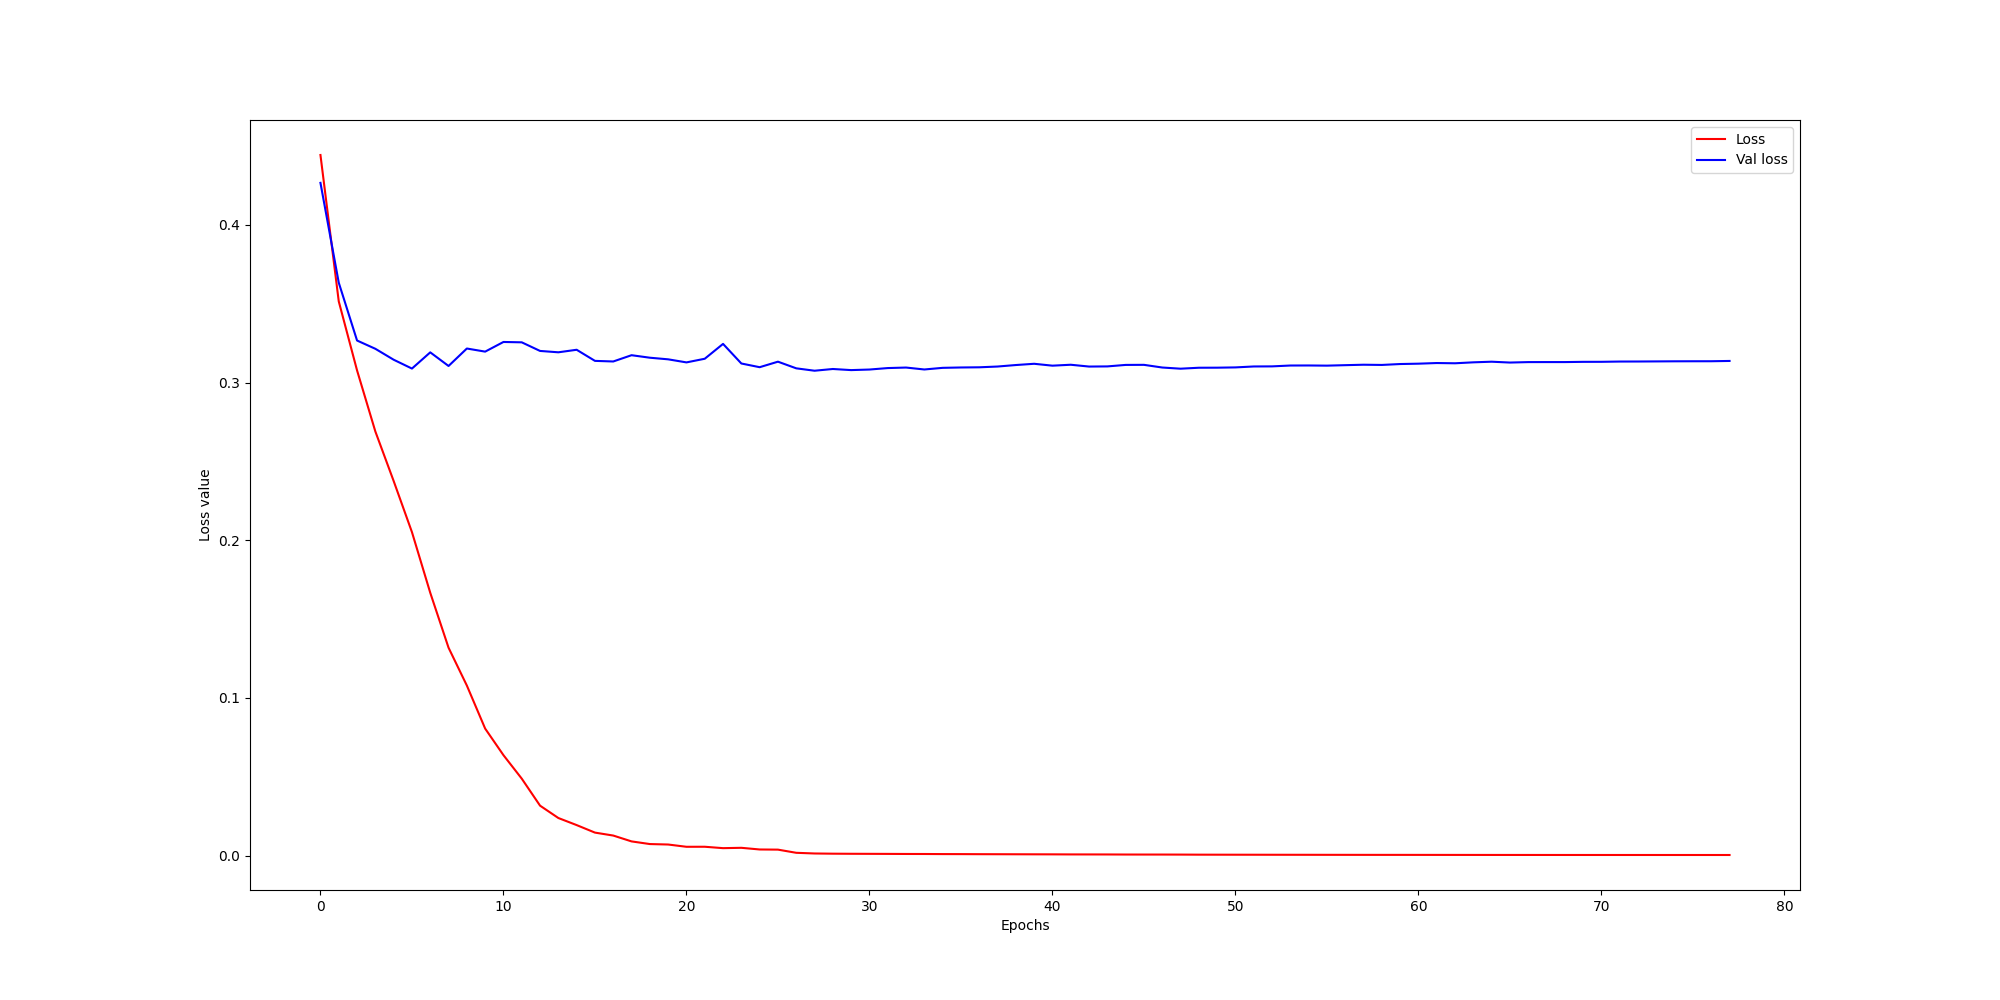
\includegraphics[width=1\linewidth]{imgs/training-76-epochs.png}
% 	\caption{Wykres uczenia}
% 	\label{fig:ucznenie}
% \end{figure}

\paragraph{Accuracy} obliczana na późniejszym etapie przy ewaluacji modelu na różnych zbiorach danych na podstawie wzoru:
$$ acc = \frac{true\_predictions}{total} $$ 

% \begin{figure}[htb]
%   \centering
% 	\begin{tabular}{@{}ll@{}}
% 	a) & b) \\
%   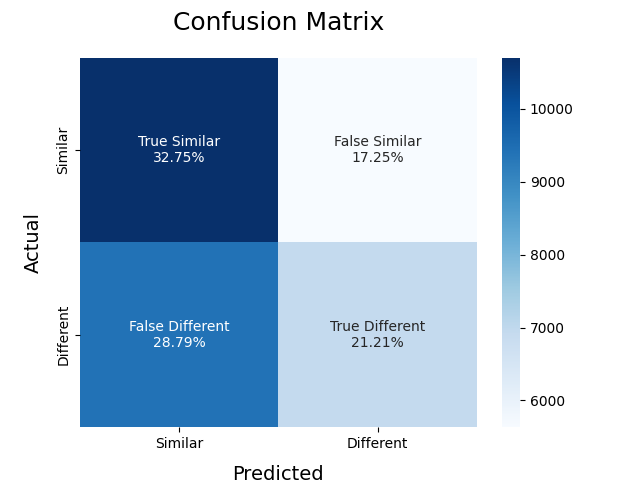
\includegraphics[width=0.475\textwidth]{imgs/celeba-learning-acc=0.5396154788145971.png} & 
% 	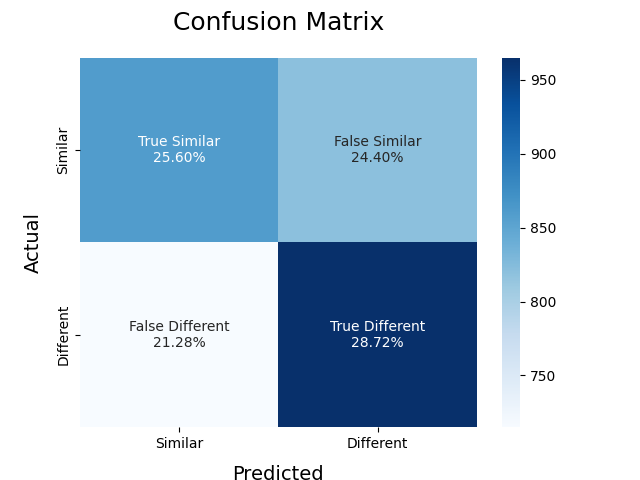
\includegraphics[width=0.475\textwidth]{imgs/lfw-learning-acc=0.5431547619047619.png}
% 	% jeśli obraki są różnej wysokości, można je wyrównać do góry stosując vtop jak niżej
% 	% \vtop{\vskip-2ex\hbox{{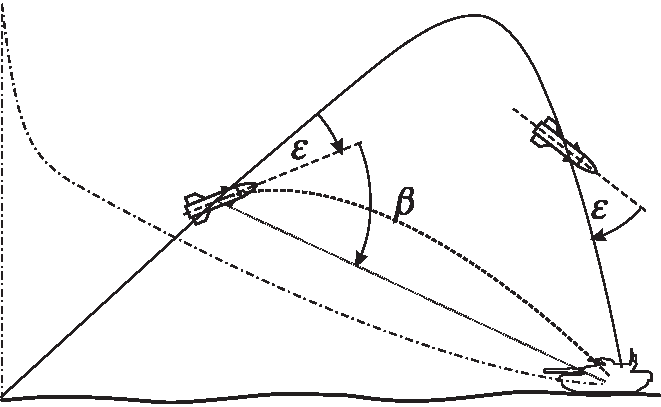
\includegraphics[width=0.475\textwidth]{rys05/beta1}}}} &
% 	% \vtop{\vskip-2ex\hbox{{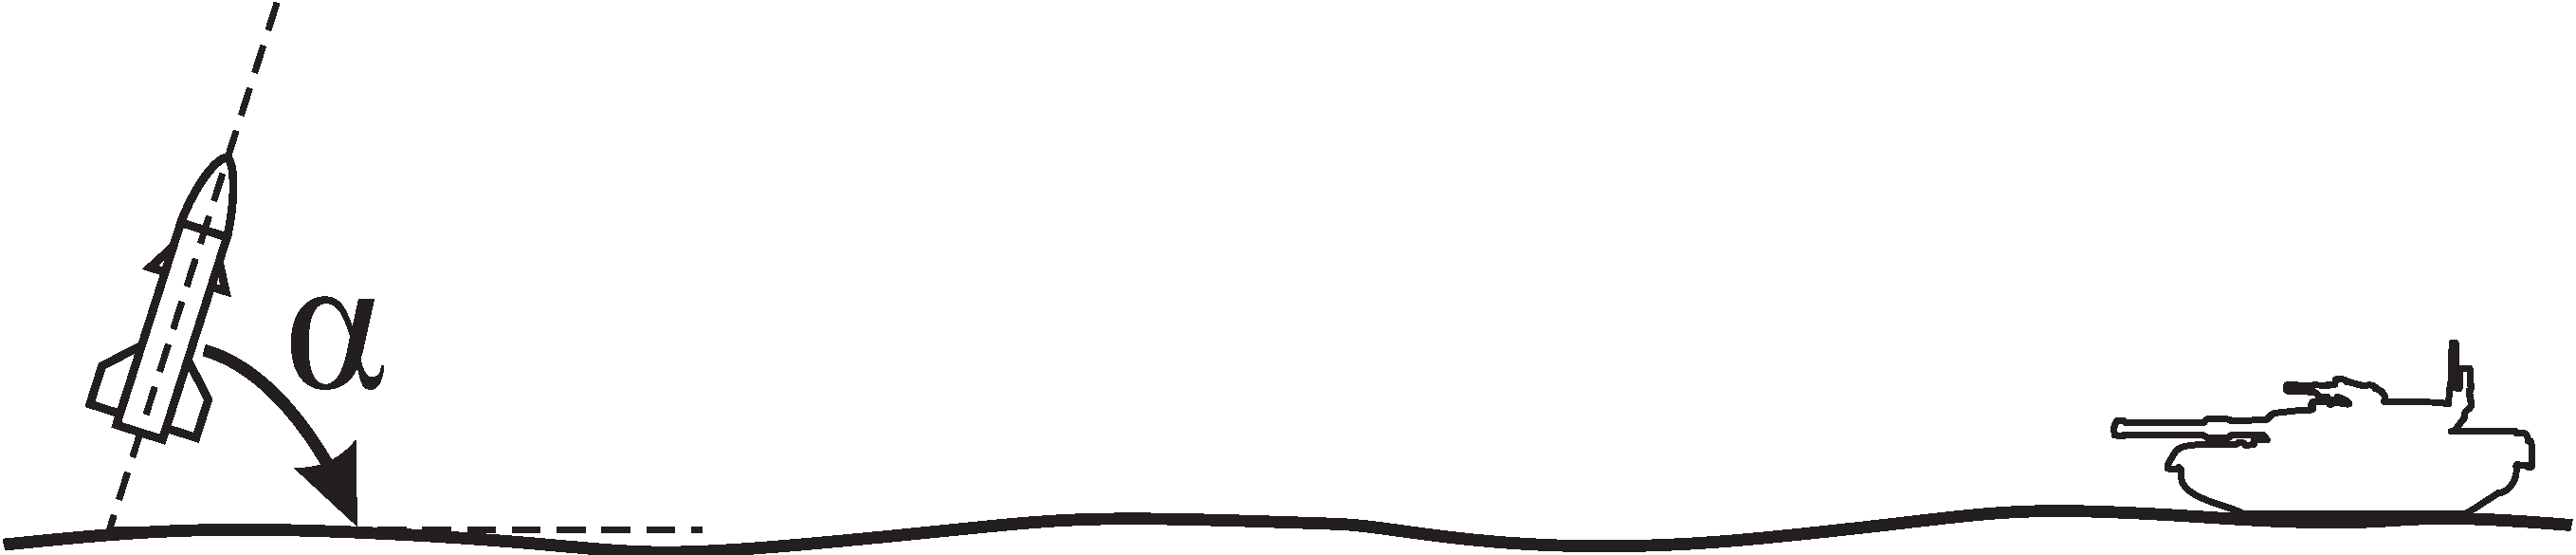
\includegraphics[width=0.475\textwidth]{rys05/alfa1}}}}  \caption{Wyznaczanie trajektorii lotu rakiety: 
% 	\end{tabular}
%   \caption{Macierz konfuzji: a) Dla zbioru CelebA, b) Dla zbioru LFW}
%   \label{fig:conf}
% \end{figure}

% Przy pomocy metryk wyznaczono, że model ma 53\% dokładność przy jednoczesnej wartości straty walidacyjnej na poziomie 0,3. Oznacza to, że model jest w dobrym stopniu dopasowany do danych walidacyjnych ale ma dokładność na niskim poziomie.

\section{Opracowanie ankiety}
Zadaniem ankiety było zbadanie doświadczeń i opinii osób na temat metod uwierzytelniania w tym takich, które wykorzystują sztuczną inteligencję. Grupa badawcza składała się z przypadkowych osób z różnych grup wiekowych o zróżnicowanym doświadczeniu z aplikacjiami internetowymi aby wyniki były obiektywne oraz zróżnicowane pod kątem opinii oraz doświadczeń. \\
Ankieta została opracowana przy pomocy aplikacji \emph{Microsoft Forms}, które jest bardzo popularnym i darmowym narzędziem do tworzenia ankiet. Oferuje możliwość personalizacji oraz tworzenia bardzo zaawansowanych kwestionariuszy pod kątem różnych typów odpowiedzi użytkowników. Dodatkowo aplikacja oferuje podgląd zebranych odpowiedzi oraz prezentację wyników w postaci rożnego rodzaju wykresów co na etapie analizy jest bardzo pomocne
\subsection{Doświadczenia z metodami uwierzytelniania i sztuczną inteligencją} Pierwsza część ankiety skupiała się na zbadaniu doświadczenia użytkowników z powszechnie dostępnymi metodami uwierzytelniania oraz ich bezpieczeństwem. Ponadto ta część miała również za zadanie zebranie danych na temat odczuć grupy badawczej na temat wykorzystania sztucznej inteligencji w zakresie bezpieczeństwa w internecie.

\begin{table}[htb]
\centering
\caption{Zbiór pytań pierwszej części ankiety}
\label{tab:ankieta-part-1}\small
\begin{tabularx}{\linewidth}{|c|X|X|} 
  \hline
Nr & Pytanie & Typ \\ 
\hline\hline
1 & Grupa wiekowa do której należysz & Jednokrotny wybór \\
2 & Ile godzin spędzasz w internecie? & Jednokrotny wybór \\
3 & Jakie urządzenie wykorzystujesz najczęściej do przebywania w internecie & Wielokrotny wybór \\
4 & Jakie jest Twoje doświadczenie z metodami uwierzytelniania & Ocena 1-5 \\
5 & W której dziedzinie najczęściej wykorzystujesz metody uwierzytelniania & Jednokrotny wybór \\
6 & Jakie metody uwierzytelniania stosujesz na codzień? & Wielokrotny wybór \\
7 & Oceń poniższe metody uwierzytelniania & Linkieta \\
8 & Czy padłeś/padłaś ofiarą włamania na konto & Tak/Nie \\
9 & W jaki sposób wykradziono Ci dane do logowania & Jednokrotny wybór \\
10 & Jaką metodę uwierzytelniania stosowałeś/stosowałaś wtedy? & Jednokrotny Wybór \\
11 & Jaki jest Twój stosunek do polityki haseł? & Ocena 1-5 \\
12 & Czy Twoim zdaniem polityka haseł ma znaczący wpływ na bezpieczeństwo? & Tak/Nie \\
13 & Dlaczego tak uważasz? & Odpowiedz tekstowa \\
14 & Czy zdarza Ci się czasem zapomnieć hasło? & Tak/Nie \\
15 & Jak często zdarza Ci się zapomnieć hasło? & Jednokrotny wybór \\
16 & Czy wykorzystanie sztucznej inteligencji jako metody uwierzytelniania mogłoby poprawić bezpieczeństwo? & Tak/Nie \\
17 & Dlaczego tak uważasz? & Odpowiedź tekstowa \\
18 & Czy mając możliwość stosowania uwierzytelniania przy pomocy rozpoznawania twarzy w aplikacjach internetowych wykorzystał/a byś taką opcję? & Tak/Nie \\
19 & Dlaczego? & Wypowiedź tekstowa \\
20 & Co Twoim zdaniem mogłoby poprawić bezpieczeństwo związane z metodami uwierzytelniania w aplikacjach internetowych? & Odpowiedź tekstowa \\
\hline
\end{tabularx}
\end{table}

\newpage
\subsection{Opinia z użytkowania platformy testowej} Druga część ankiety była odpowiedzialna za uzyskanie opinii grupy badawczej na temat zaproponowanych metod uwierzytelniania, tych tradycyjnych oraz wykorzystujących sztuczną inteligencję z zakresu rozpoznawania twarzy. Ocenie zostały poddane zarówno kwestie bezpieczeństwa oraz intuicyjność aplikacji.

\begin{table}[htb]
  \centering
  \caption{Zbiór pytań drugiej części ankiety}
  \label{tab:ankieta-part-2}\small
  \begin{tabularx}{\linewidth}{|c|X|X|} 
    \hline
  Nr & Pytanie & Typ \\ 
  \hline\hline
  1 & Czy miałeś/aś możliwość przetestować aplikację? & Tak/Nie\\
  2 & Czy Twoim zdaniem aplikacja jest bezpieczna & Tak/Nie \\
  3 & Czy wykorzystałeś/aś wszystkie dostępne metody uwierzytelniania? & Tak/Nie  \\
  4 & Oceń bezpieczeństwo zaprezentowanych metod uwierzytelniania & Linkieta \\
  5 & Co Twoim zdaniem mogłoby poprawić bezpieczeństwo aplikacji? & Odpowiedź tekstowa \\
  6 & Czy aplikacja była intuicyjna w obsłudze? & Tak/Nie \\
  7 & Co sprawiło że aplikacja była nieintuicyjna? & Odpowiedź tekstowa \\
  8 & Na jakim urządzeniu używałeś/aś aplikacji? & Jednokrotny wybór \\
  9 & Jakie masz uwagi co zaprezentowanej aplikacji? & Odpowiedź tekstowa \\
  \hline
  \end{tabularx}
  \end{table}
% \begin{enumerate}
  % \item Doświadczenia z metodami uwierzytelniania --- Składająca się z 20 pytań. 
  % \item Opinia po obsłudze platformy testowej --- Składająca sie z 9 pytań
% \end{enumerate}

% \chapter{Zalecenia dotyczące formatowania}
% Większa część niniejszego rozdziału ma charakter informacyjny. Treści w nim zawarte mają uzmysłowić czytelnikowi, jak wiele jest parametrów do ustawienia, by zredagowany dokument wyglądał ,,ładnie''. Parametry te poustawiano w szablonie. Wystarczy z niego skorzystać.

% \section{Rozmiar i układ treści na stronach dokumentu}
% Praca dyplomowa powinna być przygotowana do wydruku na papierze formatu A4 w orientacji pionowej.
% Marginesy na stronach parzystych i nieparzystych powinny być jednakowe i mieć następujące wartości:
% lewy = 25mm, prawy = 25mm, górny = 10mm, dolny = 15mm. Wielkość marginesów w szablonie sterowana jest parametrami przedstawionymi na rysunku~\ref{fig:pageLayout}. Margines dolny powinien być mierzony do linii bazowej tekstu stopki.
% %\begin{figure}[htb]
% 	%\centering
% 	%\includegraphics[width=.7\linewidth]{rys03/pageLayout2}
% 	%\caption{Kontrola marginesów i odstępów elementów na stronie} \label{fig:pageLayout}
% %\end{figure}
% \begin{figure}[htb]
% \setlayoutscale{0.43}
% \currentpage
% \drawparameterstrue
% %\drawpage
% \oddpagelayoutfalse
% \drawstock
% \caption{Układ strony nieparzystej dla dokumentu klasy \texttt{memoir}} \label{fig:pageLayout}
% \end{figure}

% Rzeczywisty układ strony zastosowany w niniejszym dokumencie przedstawiono na rysunku~\ref{fig:currentPageLayout}. Lewy i prawy margines są takie same, więc strony parzyste i nieparzyste wyglądają podobnie, z dokładnością do umiejscowienia notatek marginesowych. Taki rezultat zapewniło zastosowanie poniższych komend. 
% \begin{figure}[t]
% \setlayoutscale{0.43}
% \currentstock
% \oddpagelayouttrue
% \twocolumnlayoutfalse
% \drawmarginparstrue
% \drawparametersfalse
% \drawstock
% \caption{Rzeczywisty układ strony nieparzystej w tym dokumencie} \label{fig:currentPageLayout}
% \end{figure}

% \begin{lstlisting}[basicstyle=\footnotesize\ttfamily]
% \setlength{\headsep}{10pt} 
% \setlength{\headheight}{13.6pt} 
% \setlength{\footskip}{\headsep+\headheight}
% \setlength{\uppermargin}{\headheight+\headsep+1cm}
% \setlength{\textheight}{\paperheight-\uppermargin-\footskip-1.5cm}
% \setlength{\textwidth}{\paperwidth-5cm}
% \setlength{\spinemargin}{2.5cm}
% \setlength{\foremargin}{2.5cm}
% \setlength{\marginparsep}{2mm}
% \setlength{\marginparwidth}{2.3mm}
% \checkandfixthelayout[fixed] 
% \linespread{1}
% \setlength{\parindent}{14.5pt}
% \end{lstlisting}


% \section{Strona tytułowa}
% Stronę tytułową przygotowano starając się wypełnić zalecenia zamieszczone na stronie Wydziału Informatyki i Teleinformatyki (\url{https://wit.pwr.edu.pl/studenci/dyplomanci/praca-dyplomowa}, [dostęp dnia 16.12.2022]). Zastosowano więc pakiet \texttt{ebgaramond}. Dostarcza on klonu wymaganej czcionki \texttt{garamond}, jednak bez kształtu \texttt{slanted} i z pewnymi brakami. Na przykład zamiast literki ,,ł'' w zbiorze \texttt{EBGaramond08 Italic} renderuje się samo ,,l'' (braku tego nie ma zbiór \texttt{EBGaramond12}).  Zaletą pakietu  w porównaniu do innych jest to, że generalnie dobrze obsługiwane są w nim polskie znaki oraz że pakiet ten można znaleźć w różnych dystrybucjach latexa (\texttt{MikTeX} instaluje go automatycznie).

% Wielkości znaków użytych do wypełnienia strony tytułowej treścią są następujące:
% \begin{lstlisting}[basicstyle=\footnotesize\ttfamily]
% Politechnika Wrocławska (Garamond Bold 20pt 22pt)
% Wydział Informatyki i Teleinformatyki (Garamond Bold 16pt 18pt)
% Kierunek: Jakiś kierunek (Garamond 14pt 16pt, Garamond Bold 14pt 16pt)
% Specjalność: Jakaś specjalność (Garamond 14pt 16pt, Garamond Bold 14pt 16pt)
% {P}RACA {D}YPLOMOWA (Garamond 26pt 28pt, Garamond 24pt 26pt)
% {I}NŻYNIERSKA (Garamond 26pt 28pt, Garamond 24pt 26pt)
% Tytuł pracy w języku polskim (Garamond Bold 18pt 20pt)
% Title in English (Garamond Bold 18pt 20pt)
% % AUTOR: (Garamond 16pt 18pt) - zamarkowane
% Imię Nazwisko (Garamond Bold 16pt 18pt)
% Opiekun pracy (Garamond 14pt 16pt)
% tytuł/stopień naukowy, Imię Nazwisko (Garamond 14pt 16pt)
% %OCENA PRACY: (Garamond 16pt 18pt) - zamarkowane
% WROCŁAW, 2021 (Garamond 14pt 16pt)
% \end{lstlisting}


% \section{Główny tekst}
% Główny tekst pracy powinien być zredagowany z wykorzystaniem czcionki \texttt{Times}, typ normalny, o wysokości 12pt, z odstępem między liniami równym 14.5pt. Istnieje możliwość zmiany odstępu między liniami za pomocą komendy \verb?\linespread?, jednak zaleca się pozostawienie tego odstępu jak w niniejszym dokumencie (\verb?\linespread{1}?). Wymagania odnośnie kroju pisma pozostałych elementów (nagłówków, stopek itp.) zamieszczono w tabeli~\ref{tab:secfonts}.

% W szablonie zastosowano czcionkę \texttt{texgyre-termes} (dostarcza ją pakiet \texttt{tgtermes}). Czcionka ta jest klonem czcionki \texttt{Times}, w którym obsługiwane jest środkowoeuropejskie kodowanie znaków (podobnie jak w przypadku czcionki \texttt{ebgaramond}, dzięki czemu polskie literki nie są zlepkami dwóch znaków lecz pojedynczymi znakami).  

% Wszelkie przykłady źródeł kodu (fragmenty programów, komendy linii poleceń), nazwy plików i uruchamianych programów powinny być pisane czcionką maszynową. W szablonie czcionką maszynową jest \texttt{t1xtt}. Czcionka ta obsługuje polskie znaki. Dostarcza ją pakiet \texttt{txfonts}, który należy wcześniej zainstalować (MiKTeX zainstaluje go automatycznie podczas pierwszej kompilacji szablonu).   

% % https://en.wikibooks.org/wiki/LaTeX/Lengths
% % there are two different point sizes.  A pdf point is 1/72 inch.  A LaTeX point is 1/72.27 inch.  Thus,
% % the LaTeX point is slightly smaller than a pdf point. 

% %\texttt{baselineskip}: \printlength{\baselineskip}\\
% %\texttt{beforesecskip}: \printlength{\beforesecskip}\\
% %\texttt{aftersecskip}: \printlength{\aftersecskip}\\
% %\texttt{topskip}: \printlength{\topskip}\\
% %\texttt{fontsize}: \showFontSize\\

% \begin{table}[htb]
% \centering
% \caption{Zestawienie czcionek elementów podziału dokumentu, tekstu wiodącego, nagłówka i stopki oraz podpisów (Rozm. -- rozmiar czcionki, Odst. -- \texttt{baselineskip})}
% \label{tab:secfonts}\small
% \begin{tabularx}{\linewidth}{|ll@{\hskip 5pt}l@{\hskip 5pt}lX|} \hline
% Element & Przykład & Czcionka & Rozm. & Odst. \\ \hline\hline
% Nr rozdziału & {\huge\bfseries Rozdział 1 } & \verb?\huge\bfseries? & 25pt & 30pt \\
% Tytuł rozdziału & {\Huge\bfseries Wstęp } & \verb?\Huge\bfseries? & 30pt & 37pt\\
% Nr i tytuł sekcji & {\Large\bfseries 1.1. Wprowadzenie } & \verb?\Large\bfseries? & 17pt & 22pt \\
% Nr i tytuł podsekcji & {\large\bfseries 1.1.1. Cel szczegółowy } & \verb?\large\bfseries? &14.5pt & 18pt\\
% Tytuł podpodsekcji  & {\normalsize\bfseries Założenia } & \verb?\normalsize\bfseries? & 12pt & 14.5pt\\
% Tytuł paragrafu & {\normalsize\bfseries  Podstawy } Opis ... &  \verb?\normalsize\bfseries? & 12pt & 14.5pt\\
% Tekst wiodący & {\normalsize Niniejszy dokument ... } & \verb?\normalsize? & 12pt & 14.5pt\\
% Nagłówek strony & {\small\itshape 3.2. Czcionka wiodąca ...} & \verb?\small\itshape? & 11pt & 13.6pt \\
% Stopka strony & {\small Imię Nazwisko: ...} & \verb?\small? & 11pt & 13.6pt\\
% Podpisy tabel & {\small Tab.~3.1: Zestawienie ...} & \verb?\small? & 11pt & 13.6pt \\
% Podpisy rysunków & {\small Rys.~3.1: Oficjalny ...} & \verb?\small? & 11pt & 13.6pt\\\hline
% \end{tabularx}
% \end{table}
% %\texttt{fontsize}: \showFontSize

% Jeśli w pracy zostaną użyte otoczenia matematyczne, to w dokumencie wynikowym pojawią się dodatkowe czcionki (domyślne latexowe czcionki do wyrażeń matematycznych). Dzięki zastosowaniu opcji \texttt{extrafontsizes} w klasie \texttt{memoir} nie dość, że otrzymuje się większe czcionki (30pt), to jeszcze zamiast \texttt{Computer Modern} do wzorów matematycznych jest stosowana czcionka \texttt{Latin Modern} (wywodząca się z \texttt{Computer Modern}).
% Stąd lista wszystkich użytych czcionek może być następująca:
% \begin{lstlisting}[basicstyle=\footnotesize\ttfamily]
% EBGaramond12-Regular
% GaramondNo8-Reg-Norml
% TeXGyreTermes-Regular-Normalna
% TeXGyreTermes-Bold-Pogrubiona
% TeXGyreTermes-Italic-Normalna
% t1xtt-Nomal
% LMMathItalic12-Regular
% LMMathSymbols10-Regular
% LMMathExtension10-Regular
% LMRoman8-Regular
% \end{lstlisting}

% Aby wykorzystać te czcionki poza systemem LaTeX, wystarczy pobrać je spod adresów (ważnych na dzień
% 1.04.2016): 
% \url{https://www.ctan.org/tex-archive/fonts/cm/ps-type1/bakoma/ttf/?lang=en}, \url{http://www.gust.org.pl/projects/e-foundry/latin-modern}, \url{http://www.gust.org.pl/projects/e-foundry/tex-gyre}, \url{https://bitbucket.org/georgd/eb-garamond/downloads},
% a następnie zainstalować w systemie. Dzięki temu można będzie np.~edytować rysunki używając dokładnie tej samej czcionki, co czcionka użyta w dokumencie.

% \section{Formatowanie bloków tekstu}
% Każdy rozdział pracy powinien rozpoczynać się od nowej strony. Jej wygląd powinien być kontrolowany parametrami pokazanymi na rysunku~\ref{fig:LayChap}.
% \begin{figure}[t]
% \setlayoutscale{0.6}
% \centering
% \chapterdiagram
% \caption{Parametry sterujące wielkościami odstępów na stronie z tytułem rozdziału} 
% \label{fig:LayChap}
% \end{figure}
% W niniejszym szablonie (dokument klasy \texttt{memoir} z opcją \texttt{[12pt]}) przyjęto następujące wartości tych parametrów:
% \begin{itemize}
% \item \verb?\beforechapskip? (\printlength{\beforechapskip}) + \verb?\baselineskip? of \verb+\huge+ (30pt) + \verb+\topskip+ (\printlength{\topskip}) = 92pt (3.246cm)
% \item \verb?\midchapskip? (\printlength{\midchapskip}) + \verb?\baselineskip? of \verb+\Huge+ (37pt) = 57 pt (2.011cm)
% \item \verb?\afterchapskip? (\printlength{\afterchapskip}) + \verb+\baselineskip+ of \verb+\normalsize+ (14.5pt) = 54.5pt (1.923cm)
% \end{itemize}

% Nieco kłopotów może sprawić dobre ustawienie na stronie tytułów nienumerowanych rozdziałów oraz list generowanych automatycznie (Skróty, Spis treści, Spis rysunków, Spis tabel, Indeks rzeczowy). W szablonie w tym celu zdefiniowano nowy styl rozdziału komendami jak niżej (w szablonie są to komendy zamarkowane)
% \begin{lstlisting}[basicstyle=\footnotesize\ttfamily]
% \newlength{\linespace}
% \setlength{\linespace}{-\beforechapskip-\topskip+\headheight+\topsep}
% \makechapterstyle{noNumbered}{%
% \renewcommand\chapterheadstart{\vspace*{\linespace}}
% }
% \end{lstlisting}
% oraz dokonano przełączenia stylów rozdziałów komendami \verb?\chapterstyle{nonumbered}? oraz \verb?\chapterstyle{default}? podczas dołączania do dokumentu wymienionych nienumerowanych rozdziałów i list. Aby ,,podnieść do góry'' tytuły nienumerowanych rozdziałów (gdy jest to rzeczywiście konieczne) wystarczy odmarkować wspomniane komendy.

% Tytuły rozdziałów, sekcji, podsekcji itd.\ nie powinny kończyć się kropką. Odległości pomiędzy tekstem wiodącym a tytułem sekcji powinien być regulowany parametrami pokazanymi na rysunku~\ref{fig:LaySec}. 
% \begin{figure}[t]
% %\setlayoutscale{1}
% \runinheadfalse
% \drawparameterstrue
% \drawheading{\Large\bfseries}
% \caption{Kontrola ustawień odległości w tytułach kolejnych sekcji} 
% \label{fig:LaySec}
% \end{figure}
% Rozmiar \verb?\baselineskip? zależy od rozmiaru czcionki (zobacz tabela~\ref{tab:secfonts}), zaś \texttt{beforeskip} i \texttt{secskip} od poziomu sekcji. W niniejszym szablonie przyjęto następujące wartości tych parametrów (są to wartości dobierane elastycznie podczas kompilacji):
% \begin{itemize}
% \item \texttt{indent = 14.5pt}
% \item \texttt{parskip = \printlength{\parskip}}
% \item \texttt{beforesecskip = \printlength{\beforesecskip}}
% \item \texttt{aftersecskip = \printlength{\aftersecskip}}
% \item \texttt{beforesubsecskip = \printlength{\beforesubsecskip}}
% \item \texttt{aftersubsecskip = \printlength{\aftersubsecskip}}
% \item \texttt{beforesubsubsecskip = \printlength{\beforesubsecskip}}
% \item \texttt{aftersubsubsecskip = \printlength{\aftersubsecskip}}
% \end{itemize}

% W szablonie obowiązują również następujące wartości parametrów odpowiedzialnych za odstępy pomiędzy pływającymi figurami, tekstami oraz tekstem i figurą:
% \begin{itemize}
% \item \texttt{floatsep = \printlength{\floatsep}}
% \item \texttt{intextsep = \printlength{\intextsep}}
% \item \texttt{textfloatsep = \printlength{\textfloatsep}}
% \end{itemize}

% Pierwsza linia pierwszego akapitu w bloku (po tytule rozdziału, sekcji, podsekcji, podpodsekcji) nie może mieć wcięcia. Pierwsze linie w kolejnych akapitach już powinny mieć wcięcie równe \texttt{14.5pt}. Tekst w akapitach powinien być wyrównany z obu stron. 


% Strony powinny być numerowane numeracją ciągłą (sekwencja arabskich cyfr). Numery stron powinny być umieszczone w ich stopkach (tj.\ tak jak w niniejszym dokumencie). Wyjątkiem są tutaj pierwsze strony rozdziałów oraz strona tytułowa -- na nich numery nie powinny się pojawić.

% \section{Opisy tabel i rysunków}
% Podpisy powinny być umieszczane pod rysunkami lub nad tabelami wraz z etykietą składającą się ze skrótu Rys.\ lub Tab.\ oraz numeru. Podpisy te nie powinny mieć końcowej kropki. Numery występujący w podpisach powinny zaczynać się numerem rozdziału, po którym następuje kolejny numer rysunku lub tabeli w obrębie rozdziału. Etykieta powinna kończyć się dwukropkiem, po którym następuje tekst podpisu. Numer rozdziału powinien być rozdzielony kropką od kolejnego numeru w rysunku bądź tabeli w rozdziale (liczniki tabel i rysunków są rozłączne). Należy pamiętać o tym, żeby w całej pracy tabele miały podobny wygląd (rodzaj czcionki, ewentualne pogrubienia w nagłówku itp.). %Źródła należy podawać pod tabelą.

% \section{Przypisy dolne}
% Istnieje możliwość zamieszczania przypisów na dole strony, choć nie jest to zalecane (przykładowo~\footnote{Tekst przypisu}). Sposób parametryzowania ich wyglądu pokazano na rysunku~\ref{fig:fp}. W szablonie wykorzystano następujące, domyślne wartości tych parametrów:
% \begin{lstlisting}[basicstyle=\footnotesize\ttfamily]
% \footins = 12pt \footnotesep = 8pt
% \baselineskip = 10pt note separation = 40pt
% rule thickness = 0.4pt
% rule length = 0.25 times the \textwidth
% \end{lstlisting}
% \begin{figure}[htb]
% \setlayoutscale{0.3}
% \drawfootnote
% \caption{Parametry sterujące przypisami dolnymi} \label{fig:fp}
% \end{figure}
% %\tryfootins
% %\tryfootnotesep
% %\tryfootnotebaseline
% %\tryfootruleheight
% %\tryfootrulefrac

% %\footins = 12pt \footnotesep = 8pt
% %\baselineskip = 10pt note separation = 40pt
% %rule thickness = 0.4pt
% %rule length = 0.25 times the \textwidth

% \section{Formatowanie spisu treści}
% W klasie \texttt{memoir} istnieją komendy pozwalające dość dobrze zarządzać wyglądem spisu treści. Na rysunku~\ref{fig:ltoc} pokazano, za pomocą jakich parametrów można wpływać na finalną jego postać. W szablonie wykorzystano następujące, domyślne ich wartości:
% \begin{lstlisting}[basicstyle=\footnotesize\ttfamily]
% indent = 18pt 
% numwidth = 28pt
% \@tocrmarg = 31pt 
% \@pnumwidth = 19pt
% \@dotsep = 4.5
% \end{lstlisting}

% \begin{figure}[h]
% \setlayoutscale{0.5}
% \drawtoc
% \caption{Parametryzacja wyglądu spisu treści} \label{fig:ltoc}
% \end{figure}

% %\begin{figure}
% %\setlayoutscale{0.8}
% %\currenttoc
% %\drawparametersfalse
% %\drawtoc
% %\caption{Parametry definiujące postać spisu treści w niniejszym szablonie} \label{fig:thistoc}
% %\end{figure}

% \section{Formatowanie list wyliczeniowych i wypunktowań}
% Standardowo sposób formatowania list można parametryzować jak pokazano na rysunku~\ref{fig:listlay}. Jednak czasem trudno poradzić sobie z niektórymi rzeczami, jak np.~znakami wypunktowania. Dlatego w szablonie wykorzystano pakiet \texttt{enumi}. Pozwala on na łatwe zarządzanie wyglądem list. W szablonie zastosowano następujące globalne ustawienia dla tego pakietu:
% \begin{lstlisting}[basicstyle=\footnotesize\ttfamily]
% \usepackage{enumitem} 
% \setlist{noitemsep,topsep=4pt,parsep=0pt,partopsep=4pt,leftmargin=*} 
% \setenumerate{labelindent=0pt,itemindent=0pt,leftmargin=!,label=\arabic*.} 
% \setlistdepth{4} 
% \setlist[itemize,1]{label=$\bullet$} 
% \setlist[itemize,2]{label=\normalfont\bfseries\textendash}
% \setlist[itemize,3]{label=$\ast$}
% \setlist[itemize,4]{label=$\cdot$}
% \renewlist{itemize}{itemize}{4}
% \end{lstlisting}
% \begin{figure}[h]
% \centering
% \setlayoutscale{0.4}
% \drawparameterstrue
% \drawlist
% \caption{Parametryzacja list wyliczeniowych i wypunktowań}\label{fig:listlay}
% \end{figure}

% W~podrozdziale~\ref{sec:Styl} pokazano przykład wykorzystania możliwości komend oferowanych w~pakiecie \texttt{enumi}.

% \section{Wzory matematyczne}
% Wzory matematyczne, jeśli mają być osobnymi formułami, powinny być wycentrowane, z~numeracją umieszczoną na końcu linii i ujętą w okrągłe nawiasy (zobacz równanie (\ref{eq:xdx})). Numery równań powinny zawierać numer rozdziału oraz kolejny numer równania w obrębie rozdziału (podobnie jak przy numerowaniu rysunków i tabel). Spełnienie tych warunków zapewnia otoczenie \verb?equation?. Nie wszystkie formuły trzeba numerować (nienumerowane wzory można osiągnąć stosując otoczenie \verb?\equation*?). Właściwie należy numerować tylko te, do których tworzy się jakieś odniesienia w tekście. Jeśli wzory umieszczane są w linijce tekstu, to można zastosować otoczenie matematyczne inline, jak w~przykładzie $\int_{0}^{10\nu\sum i}{x dx}$ (wyprodukowanym komendą \verb?$\int_{0}^{10\nu\sum i}{x dx}$?). Tylko że wtedy może dojść do rozszerzenia odstępów pomiędzy liniami tekstu (aby zmieścił się wzór).
% \begin{equation}\label{eq:xdx}
% \int_{0}^{10\nu\sum i}{x dx}
% \end{equation}